\documentclass[11pt,a4paper]{article}

\usepackage[utf8]{inputenc}
\usepackage[T1]{fontenc}
\usepackage{mathpazo}
\usepackage[scaled=0.92]{helvet}
\usepackage[margin=1in]{geometry}
\usepackage{graphicx}
\usepackage{amsmath,amssymb,amsfonts}
\usepackage{booktabs}
\usepackage{tabularx}
\usepackage{setspace}
\usepackage{titlesec}
\usepackage{fancyhdr}
\usepackage{float}
\usepackage{caption}
\usepackage{microtype}
\usepackage{tikz}
\usepackage{xcolor}
\usepackage[hidelinks]{hyperref}

\usetikzlibrary{shapes.geometric, arrows.meta, positioning, calc, matrix, fit, backgrounds}

\setstretch{1.15}
\setlength{\parindent}{0pt}
\setlength{\parskip}{0.8em}
\sloppy

\titleformat{\section}{\normalfont\large\bfseries\sffamily}{\thesection}{1em}{}
\titleformat{\subsection}{\normalfont\normalsize\bfseries\sffamily}{\thesubsection}{1em}{}
\titleformat{\subsubsection}{\normalfont\normalsize\itshape\sffamily}{\thesubsubsection}{1em}{}

\pagestyle{fancy}
\fancyhf{}
\fancyhead[L]{\small\sffamily Arsitektur Berlapis Sistem Kontrol Versi}
\fancyhead[R]{\small\sffamily\thepage}
\renewcommand{\headrulewidth}{0.4pt}

\captionsetup{font=small,labelfont=bf,labelsep=period}

\renewenvironment{abstract}
{\small
	\begin{center}\textbf{\sffamily Abstrak}\end{center}
	\begin{quote}}
	{\end{quote}}

\lstdefinestyle{code}{
	basicstyle=\ttfamily\small,
	frame=single,
	rulecolor=\color{black},
	breaklines=true,
	showstringspaces=false,
	columns=fullflexible,
	keepspaces=true,
	framesep=6pt,
	aboveskip=1em,
	belowskip=1em,
	xleftmargin=0pt
}

\lstdefinestyle{out}{
	basicstyle=\ttfamily\small,
	frame=tb,
	rulecolor=\color{black},
	breaklines=true,
	showstringspaces=false,
	columns=fullflexible,
	keepspaces=true,
	framesep=4pt,
	aboveskip=1em,
	belowskip=1em
}

\title{\vspace{-1.5cm}\textbf{\sffamily\LARGE Arsitektur Berlapis Sistem Kontrol Versi dalam Rust\\ Membangun libvctrl dari Nol}}
\author{
	\textbf{Muhammad Riduwan Khafidi} \\
	\small Program Studi Teknik Rekayasa Perangkat Lunak \\
	\small Politeknik Negeri Batam \\
	\small \texttt{4342611034@students.polibatam.ac.id}
}
\date{\small\today}

\begin{document}

\maketitle
\thispagestyle{empty}

\begin{abstract}
	Sistem kontrol versi modern seperti Git menopang kolaborasi perangkat lunak global, namun arsitektur internalnya jarang dibedah dalam literatur berbahasa Indonesia. Makalah ini membedah libvctrl, sebuah workspace Rust dengan enam crate publik yang membangun sistem kontrol versi dari nol menggunakan arsitektur berlapis yang ketat. Makalah menyajikan delapan visualisasi TikZ yang mencakup pemetaan lapisan, graf dependensi, model objek, pohon Merkle, siklus content addressing, perbandingan penyimpanan, pipeline kodek, dan timeline studi kasus. Setiap lapisan dibahas dengan analogi konkret, contoh berangka, dan penjelasan mengapa pemisahan kontrak dari implementasi menjadi fondasi yang dapat diuji secara independen. Melalui kerangka ini, pembaca memperoleh mental model untuk membangun sistem serupa atau membaca kode sumber VCS mana pun.
\end{abstract}

\section{Pendahuluan}

\subsection{Analogi Pembuka: Pabrik Elektronik dengan Tujuh Divisi}

Bayangkan sebuah pabrik elektronik yang memproduksi ponsel. Pabrik itu punya tujuh divisi yang bekerja berurutan, tetapi dengan batas yang tegas. Divisi pertama menetapkan standar: ukuran sekrup harus M2, bukan M3; ketebalan baterai harus 4 milimeter; antena harus punya impedansi 50 ohm. Divisi kedua merancang rangkaian sesuai standar itu. Divisi ketiga membuat komponen dasar: resistor, kapasitor, chip. Divisi keempat merakit papan sirkuit. Divisi kelima mengemas ponsel jadi unit siap jual. Divisi keenam melayani pelanggan: panduan, garansi, servis. Divisi ketujuh mengelola pabrik secara keseluruhan.

Yang penting: divisi pertama tidak peduli ponselnya warna apa. Divisi ketiga tidak peduli ponselnya dijual ke mana. Divisi keenam tidak peduli chip apa yang dipakai. Setiap divisi hanya berkomunikasi dengan divisi tetangga melalui kontrak tertulis. Jika chip diganti dari ARM ke RISC-V, divisi perakitan tetap sama selama pin dan tegangan sesuai kontrak. Jika layanan pelanggan ditambah fitur, divisi perakitan tidak perlu disentuh.

libvctrl mengikuti pola yang sama untuk sistem kontrol versi. Enam crate publik dan satu backend opsional membentuk tujuh divisi yang tidak saling mencampuri.

\subsection{Mengapa Topik Ini Penting}

Seorang pengembang yang mengerti cara Git disusun bisa mendiagnosis masalah dengan lebih cepat. Ketika \texttt{git fsck} melaporkan \textit{dangling commit}, pengembang yang paham pohon objek bisa menelusuri ke mana commit itu seharusnya menempel. Ketika \texttt{git log} terasa lambat, pengembang yang paham \texttt{ObjectStore} bisa curiga pada konkatenasi file di \texttt{.git/objects}. Tanpa mental model arsitektur, semua diagnosis berhenti pada tebakan.

Selain itu, arsitektur berlapis adalah pola yang dapat dipakai di domain lain. Sistem basis data memisahkan parser dari planner dari executor dari storage. Sistem build memisahkan dependensi dari kompilasi dari linking. Sistem paket memisahkan manifest dari resolver dari fetcher dari installer. Setiap domain punya masalah yang sama: bagaimana memisahkan aturan dari implementasi agar satu bagian bisa diganti tanpa merusak yang lain.

Rust sebagai bahasa implementasi memberi jaminan keamanan memori yang tidak dimiliki C, bahasa utama Git. libvctrl memakai Rust untuk alasan yang sama seperti sistem lain memilih Rust pada 2024 ke atas: menghilangkan kelas bug memori tanpa mengorbankan performa. Kombinasi Rust dan arsitektur berlapis adalah kombinasi yang layak dipelajari.

\subsection{Peta Pembahasan}

Makalah ini dibagi menjadi sembilan bagian utama. Bagian kedua membahas tujuh lapisan arsitektur dan mengapa pemisahan kontrak dari implementasi menjadi fondasi. Bagian ketiga membahas model objek VCS: \texttt{Blob}, \texttt{Tree}, \texttt{Commit}, \texttt{Tag}, dan \texttt{Hash}. Bagian keempat membahas content addressing dengan SHA-512 dan mengapa fungsi hash kriptografis dipakai alih-alih CRC. Bagian kelima membahas kodek biner dan backend penyimpanan. Bagian keenam menyandingkan seluruh lapisan dalam tabel perbandingan. Bagian ketujuh memuat studi kasus delapan langkah membangun commit pertama. Bagian kedelapan dan kesembilan memberi daftar kesalahan umum dan lembar rujukan cepat. Bagian kesepuluh menutup dengan tiga prinsip.

\section{Tujuh Lapisan Arsitektur}

\subsection{Mengapa Tujuh, Bukan Tiga}

Sebuah sistem kontrol versi bisa saja ditulis sebagai satu binary monolitik. Itu pilihan yang lebih sederhana pada awalnya, tetapi membawa tiga biaya yang tidak terlihat sampai sistem membesar.

Pertama, pengujian menjadi lambat. Setiap kali ingin menguji \texttt{ObjectStore}, harus ada filesystem sungguhan. Setiap kali ingin menguji \texttt{Decoder}, harus ada encoder yang sudah jalan. Tidak ada cara menguji komponen secara terisolasi.

Kedua, penggantian backend menjadi mustahil. Jika ingin menyimpan objek di SQLite sebagai ganti filesystem, seluruh kode perintah di atas harus ditulis ulang karena tidak ada batas yang jelas antara "cara menyimpan" dan "cara memakai".

Ketiga, dokumentasi menjadi kabur. Pembaca yang ingin memahami apa itu \texttt{ObjectStore} harus membaca kode penyimpanan, bukan membaca kontrak.

Tujuh lapisan libvctrl menjawab ketiga masalah itu dengan satu prinsip: setiap lapisan hanya bergantung ke lapisan di bawahnya, dan hanya melalui kontrak tertulis. Gambar~\ref{fig:layers} memetakan ketujuh lapisan itu.

\begin{figure}[H]
	\centering
	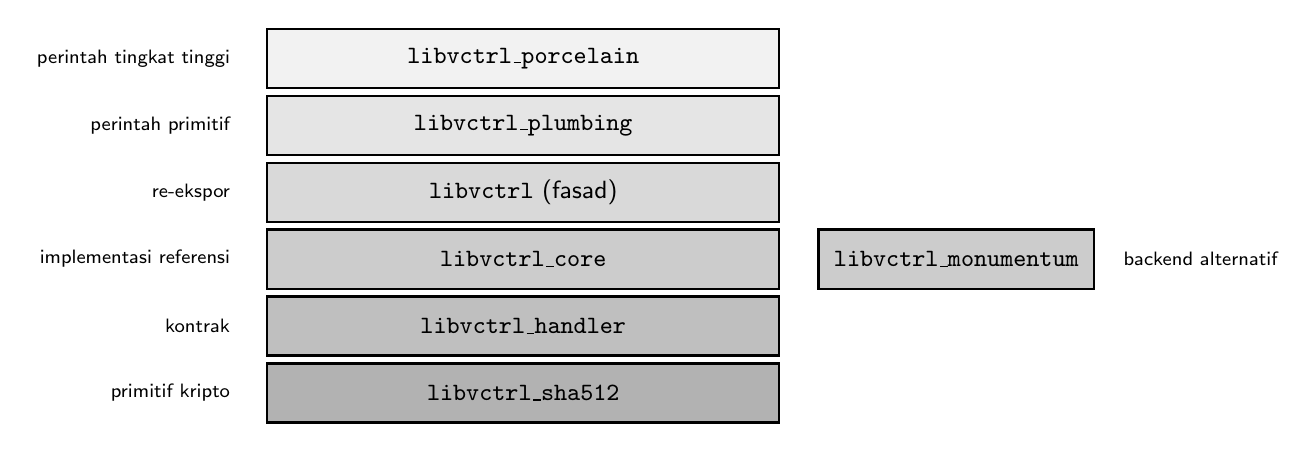
\begin{tikzpicture}[
			layer/.style={rectangle, draw=black, thick, minimum width=6.5cm, minimum height=0.75cm, align=center, font=\sffamily\small},
			lbl/.style={font=\scriptsize\sffamily, anchor=east}
		]
		\node[layer, fill=black!5]  (po) at (0, 3.5)  {\texttt{libvctrl\_porcelain}};
		\node[layer, fill=black!10] (pm) at (0, 2.65) {\texttt{libvctrl\_plumbing}};
		\node[layer, fill=black!15] (fd) at (0, 1.8)  {\texttt{libvctrl} (fasad)};
		\node[layer, fill=black!20] (co) at (0, 0.95) {\texttt{libvctrl\_core}};
		\node[layer, fill=black!25] (hd) at (0, 0.1)  {\texttt{libvctrl\_handler}};
		\node[layer, fill=black!30] (sh) at (0, -0.75){\texttt{libvctrl\_sha512}};

		\node[layer, fill=black!20, minimum width=3.5cm] (mo) at (5.5, 0.95) {\texttt{libvctrl\_monumentum}};

		\node[lbl] at (-3.6, 3.5)  {perintah tingkat tinggi};
		\node[lbl] at (-3.6, 2.65) {perintah primitif};
		\node[lbl] at (-3.6, 1.8)  {re-ekspor};
		\node[lbl] at (-3.6, 0.95) {implementasi referensi};
		\node[lbl] at (-3.6, 0.1)  {kontrak};
		\node[lbl] at (-3.6, -0.75){primitif kripto};

		\node[font=\scriptsize\sffamily, anchor=west] at (7.5, 0.95) {backend alternatif};
	\end{tikzpicture}
	\caption{Tujuh lapisan arsitektur libvctrl. Enam lapisan membentuk tumpukan utama; \texttt{libvctrl\_monumentum} adalah backend opsional yang duduk sejajar dengan \texttt{libvctrl\_core}.}
	\label{fig:layers}
\end{figure}

Cara membaca Gambar~\ref{fig:layers}: gambar ini menampilkan enam kotak bertumpuk di sisi kiri, dari \texttt{libvctrl\_porcelain} di atas sampai \texttt{libvctrl\_sha512} di bawah. Setiap kotak punya latar abu-abu yang sedikit lebih gelap dari kotak di atasnya. Di sebelah kanan tumpukan, sejajar dengan kotak \texttt{libvctrl\_core}, ada kotak ketujuh berlabel \texttt{libvctrl\_monumentum} yang lebih sempit. Di sisi kiri setiap kotak ada label peran singkat. Inti pesan gambar ini adalah tujuh lapisan dengan tanggung jawab terpisah, di mana backend alternatif dapat menggantikan lapisan implementasi tanpa mengubah lapisan lain.

\subsection{Peran Setiap Lapisan}

Lapisan \texttt{libvctrl\_sha512} hanya berisi primitif kriptografi: SHA-512, HMAC-SHA512, HKDF-SHA512, dan SHA-384 opsional. Ia tidak tahu apa itu commit, tree, atau blob. Ia hanya tahu cara mengubah byte menjadi hash 64 byte.

Lapisan \texttt{libvctrl\_handler} hanya berisi kontrak: trait, tipe data, konstanta, dan fungsi validasi. Ia tidak berisi satu pun implementasi konkret. Ia mendefinisikan apa itu \texttt{Blob}, apa itu \texttt{ObjectStore}, apa itu \texttt{Encoder}, tanpa menentukan bagaimana semuanya diwujudkan.

Lapisan \texttt{libvctrl\_core} berisi implementasi referensi: kodek biner, builder, hasher adapter, dan penyimpanan in-memory. Ia mengimplementasikan setiap trait dari \texttt{libvctrl\_handler}.

Lapisan \texttt{libvctrl} adalah fasad. Ia tidak berisi logika apa pun; setiap item publiknya adalah re-ekspor. Tujuannya hanya menyatukan tiga crate fondasi (\texttt{handler}, \texttt{core}, \texttt{sha512}) dalam satu namespace.

Lapisan \texttt{libvctrl\_plumbing} berisi perintah primitif seperti \texttt{cat-file}. Ia memakai \texttt{libvctrl\_core} sebagai backend, tetapi tidak menyembunyikan langkah apa pun.

Lapisan \texttt{libvctrl\_porcelain} berisi perintah tingkat tinggi yang membungkus plumbing menjadi alur kerja yang mudah dipakai. Contohnya adalah \texttt{commit} yang melakukan encode, hash, dan store sekaligus.

Lapisan \texttt{libvctrl\_monumentum} adalah backend alternatif: implementasi \texttt{ObjectStore} dan \texttt{RefStore} yang menyimpan data di mesin penyimpanan \texttt{monumentum}, bukan di \texttt{HashMap}. Ia duduk sejajar dengan \texttt{libvctrl\_core} karena sama-sama mengimplementasikan kontrak dari \texttt{libvctrl\_handler}.

\subsection{Arah Dependensi yang Satu Arah}

Arah dependensi bersifat satu arah dan wajib. Gambar~\ref{fig:deps} menunjukkan graf lengkapnya.

\begin{figure}[H]
	\centering
	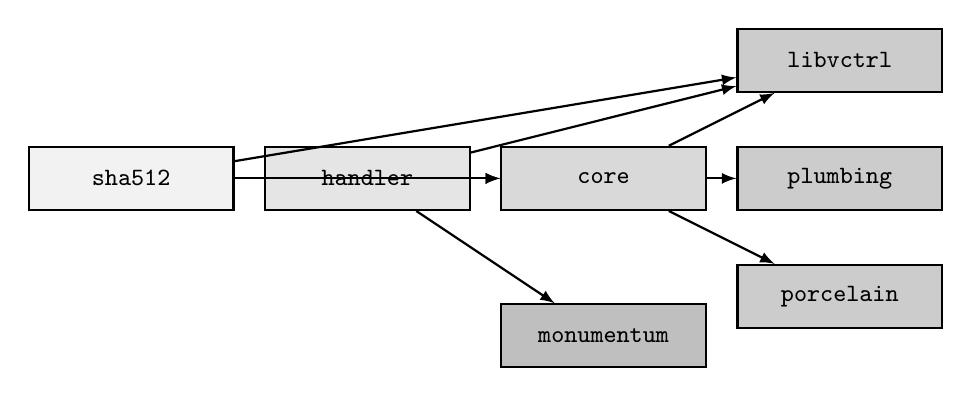
\begin{tikzpicture}[
			crate/.style={rectangle, draw=black, thick, fill=white, minimum width=2.6cm, minimum height=0.8cm, align=center, font=\ttfamily\small},
			edge/.style={draw, thick, -latex}
		]
		\node[crate, fill=black!5]  (sha) at (-3, 0)  {sha512};
		\node[crate, fill=black!10] (hd)  at (0, 0)   {handler};
		\node[crate, fill=black!15] (co)  at (3, 0)   {core};
		\node[crate, fill=black!20] (fd)  at (6, 1.5) {libvctrl};
		\node[crate, fill=black!20] (pm)  at (6, 0)   {plumbing};
		\node[crate, fill=black!20] (po)  at (6, -1.5){porcelain};
		\node[crate, fill=black!25] (mo)  at (3, -2)  {monumentum};

		\draw[edge] (sha) -- (co);
		\draw[edge] (hd) -- (co);
		\draw[edge] (hd) -- (fd);
		\draw[edge] (co) -- (fd);
		\draw[edge] (sha) -- (fd);
		\draw[edge] (co) -- (pm);
		\draw[edge] (co) -- (po);
		\draw[edge] (hd) -- (mo);
	\end{tikzpicture}
	\caption{Graf dependensi antar crate libvctrl. Panah hanya mengalir satu arah dan tidak pernah membentuk siklus.}
	\label{fig:deps}
\end{figure}

Cara membaca Gambar~\ref{fig:deps}: gambar ini menampilkan tujuh kotak bernama crate. \texttt{sha512} dan \texttt{handler} di paling kiri tidak punya panah masuk, artinya keduanya adalah fondasi yang tidak bergantung ke crate lain. \texttt{core} menerima panah dari keduanya. \texttt{libvctrl} menerima panah dari tiga crate fondasi sekaligus. \texttt{plumbing} dan \texttt{porcelain} menerima panah dari \texttt{core}. \texttt{monumentum} menerima panah dari \texttt{handler}. Tidak ada panah yang mundur. Inti pesan gambar ini adalah arah dependensi ketat satu arah dan tidak ada siklus.

Arah satu arah ini bukan sekadar konvensi. Jika \texttt{handler} sampai bergantung ke \texttt{core}, seluruh sistem akan menjadi satu kesatuan monolitik dan kehilangan seluruh manfaat pemisahan. Jika \texttt{core} sampai bergantung ke \texttt{plumbing}, maka perintah-perintah di atasnya tidak dapat diuji secara terpisah. Arah dependensi yang satu arah adalah fondasi dari seluruh klaim modularitas arsitektur ini.

\subsection{Mengapa Kontrak Terpisah dari Implementasi}

Lapisan \texttt{libvctrl\_handler} hanya berisi trait, tipe, konstanta, dan fungsi validasi. Keputusan ini punya tiga konsekuensi.

Pertama, pengujian menjadi mungkin tanpa backend. Setiap kali ingin menguji \texttt{ObjectStore}, cukup menulis struct kosong yang mengimplementasikan trait dengan perilaku minimal. Pengujian berjalan dalam hitungan milidetik, bukan detik.

Kedua, penggantian backend menjadi murah. Ketika \texttt{libvctrl\_monumentum} ditulis, ia hanya perlu mengimplementasikan dua trait: \texttt{ObjectStore} dan \texttt{RefStore}. Seluruh kode perintah di atasnya tidak tahu bahwa backend berubah.

Ketiga, dokumentasi menjadi jelas. Setiap trait punya docstring yang menjelaskan kontraknya tanpa perlu menjelaskan implementasinya.

\subsection{Ringkasan Tujuh Crate}

\begin{table}[H]
	\centering
	\caption{Ringkasan tujuh crate pada workspace libvctrl.}
	\label{tab:crates}
	\footnotesize
	\begin{tabularx}{\textwidth}{l X X}
		\toprule
		Crate                         & Peran                                  & Dependensi            \\
		\midrule
		\texttt{libvctrl\_sha512}     & Primitif kriptografi (SHA, HMAC, HKDF) & tidak ada             \\
		\texttt{libvctrl\_handler}    & Kontrak: trait, tipe, validasi         & tidak ada             \\
		\texttt{libvctrl\_core}       & Implementasi referensi                 & handler, sha512       \\
		\texttt{libvctrl}             & Fasad: re-ekspor tiga crate fondasi    & handler, core, sha512 \\
		\texttt{libvctrl\_plumbing}   & Perintah primitif                      & core                  \\
		\texttt{libvctrl\_porcelain}  & Perintah tingkat tinggi                & plumbing              \\
		\texttt{libvctrl\_monumentum} & Backend penyimpanan alternatif         & handler, monumentum   \\
		\bottomrule
	\end{tabularx}
\end{table}

\section{Model Objek VCS}

\subsection{Mengapa Empat Tipe, Bukan Satu}

Jika seluruh data disimpan sebagai byte stream tanpa tipe, sistem tidak bisa membedakan file dari direktori, atau direktori dari commit. Setiap operasi harus menebak tipe dari isinya, yang lambat dan rawan salah. Object store modern memecah data menjadi empat tipe dengan peran jelas: \texttt{Blob}, \texttt{Tree}, \texttt{Commit}, dan \texttt{Tag}. Gambar~\ref{fig:types} menunjukkan keempatnya.

\begin{figure}[H]
	\centering
	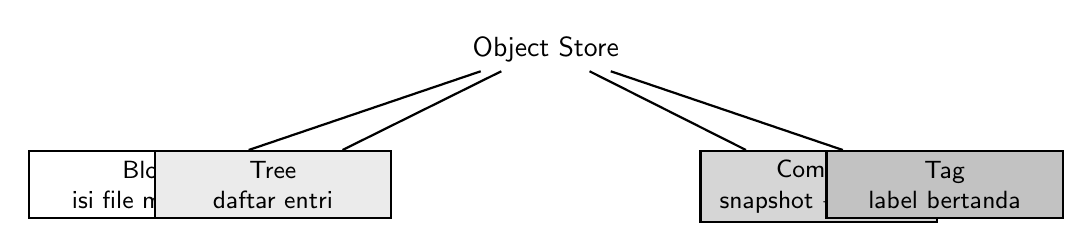
\begin{tikzpicture}[
			node distance=0.5cm and 0.8cm,
			cat/.style={rectangle, draw=black, thick, fill=white, minimum width=3cm, minimum height=0.85cm, align=center, font=\sffamily\small},
			line/.style={draw, thick}
		]
		\node[font=\sffamily] (root) at (0, 1) {Object Store};
		\node[cat, fill=white, below left=1cm and 2.5cm of root] (b) {Blob \\ isi file mentah};
		\node[cat, fill=black!8, below left=1cm and 0.9cm of root] (t) {Tree \\ daftar entri};
		\node[cat, fill=black!16, below right=1cm and 0.9cm of root] (c) {Commit \\ snapshot + parent};
		\node[cat, fill=black!24, below right=1cm and 2.5cm of root] (g) {Tag \\ label bertanda};

		\draw[line] (root) -- (b);
		\draw[line] (root) -- (t);
		\draw[line] (root) -- (c);
		\draw[line] (root) -- (g);
	\end{tikzpicture}
	\caption{Empat tipe objek pada content-addressable object store.}
	\label{fig:types}
\end{figure}

Cara membaca Gambar~\ref{fig:types}: gambar ini menampilkan satu kotak pusat berlabel Object Store, dengan empat kotak bercabang ke bawah. Cabang paling kiri berlabel Blob dengan keterangan isi file mentah. Cabang kedua berlabel Tree dengan keterangan daftar entri. Cabang ketiga berlabel Commit dengan keterangan snapshot dan parent. Cabang paling kanan berlabel Tag dengan keterangan label bertanda. Setiap cabang punya latar abu-abu yang berbeda, dari putih ke abu-abu tua. Inti pesan gambar ini adalah object store dibagi menjadi empat tipe dengan tanggung jawab berbeda.

\subsection{Blob: Isi File Tanpa Nama}

\texttt{Blob} adalah singkatan dari \textit{binary large object}. Isinya adalah byte mentah dari sebuah file, tanpa nama, tanpa path, tanpa metadata apa pun. Blob tidak tahu namanya sendiri; ia hanya tahu isinya.

Pemisahan nama dari isi adalah kunci deduplikasi. Jika dua file bernama \texttt{notes.txt} dan \texttt{backup.txt} berisi hal yang sama persis, keduanya merujuk ke blob yang sama. Sistem menyimpan satu blob, bukan dua. Karena blob tidak menyimpan nama, cara sistem menemukan blob adalah melalui \texttt{Tree}.

Konstruksi blob memakai konstruktor fallible. Jika isi melebihi batas \texttt{MAX\_BLOB\_SIZE}, konstruksi gagal dan mengembalikan \texttt{VctrlError}. Inilah contoh bagaimana kontrak dipaksakan di batas sistem.

\begin{lstlisting}[style=code]
use libvctrl::{Blob, VctrlError};

fn main() -> Result<(), VctrlError> {
    let data = b"hello, vcs".to_vec();
    let blob = Blob::new(data)?;
    println!("size = {}", blob.size());
    Ok(())
}
\end{lstlisting}

\begin{lstlisting}[style=out]
size = 10
\end{lstlisting}

Jika isi melebihi \texttt{MAX\_BLOB\_SIZE} (100 MiB), \texttt{Blob::new} mengembalikan \texttt{ExceededMaxSize}. Pemanggil tidak bisa membuat blob raksasa secara tidak sengaja.

\subsection{Tree: Daftar Entri Direktori}

\texttt{Tree} adalah satu tingkat direktori. Isinya adalah daftar entri, di mana setiap entri memiliki tiga komponen: nama, \texttt{EntryKind} (file biasa, executable, symlink, subdirektori, submodule), dan hash dari objek target.

Tree adalah tempat nama dan isi dipertemukan kembali. Sebuah blob bisa dirujuk oleh banyak tree dengan nama berbeda, dan sebuah tree bisa merujuk banyak blob dengan nama berbeda. Pada konstruksi tree, entri diurutkan dengan aturan yang sama seperti Git: nama diurutkan berdasarkan byte, dan jika nama sama persis, tree diurutkan seolah namanya ditambahi \texttt{/}.

\begin{lstlisting}[style=code]
use libvctrl::{EntryKind, Hash, Tree, TreeEntry};

let hash = Hash::from_bytes(&[0u8; 64])?;
let e = TreeEntry::new("a.txt".to_string(), EntryKind::Blob, hash)?;
let tree = Tree::new(vec![e])?;
println!("entries = {}", tree.len());
\end{lstlisting}

\begin{lstlisting}[style=out]
entries = 1
\end{lstlisting}

\subsection{Commit: Snapshot dengan Sejarah}

\texttt{Commit} adalah snapshot dari seluruh tree di root proyek pada satu titik waktu, ditambah satu atau lebih parent yang menunjuk ke commit sebelumnya. Sebuah commit menyimpan hash tree, daftar parent, author, committer, message, dan metadata opsional seperti timestamp dan encoding.

Perbedaan antara tree dan commit adalah perbedaan antara "bagaimana isi direktori saat ini" dan "mengapa isi itu seperti ini". Tree hanya menyimpan keadaan. Commit menyimpan keadaan plus alasannya.

\subsection{Tag: Label yang Bisa Ditandatangani}

\texttt{Tag} adalah label yang menunjuk ke objek lain, biasanya commit. Ada dua jenis: lightweight dan annotated. Lightweight hanyalah alias, sedangkan annotated adalah objek tersendiri yang menyimpan nama tag, hash target, tagger, pesan, dan tanda tangan kriptografis opsional.

Annotated tag adalah satu-satunya objek yang dirancang untuk ditandatangani. Tanda tangannya membuktikan bahwa tag dibuat oleh pemegang kunci privat, bukan oleh siapa pun yang bisa menulis ke repositori.

\subsection{Hash sebagai Alamat}

\texttt{Hash} adalah tipe fixed-size 64 byte. Ia mewakili alamat konten dari sebuah objek, dihitung dengan SHA-512 atas byte hasil encode objek tersebut. Karena hash adalah tipe \texttt{Copy}, ia dapat dipakai sebagai kunci pada \texttt{HashMap} tanpa cloning.

Hash menyimpan array \texttt{[u8; HASH\_LENGTH]}, yang membuat setiap nilai hash punya ukuran yang sama persis. Ukuran tetap inilah yang membuat \texttt{HashMap} dapat menyimpan jutaan objek tanpa fragmentasi.

\subsection{Pohon Merkle: Mengapa Satu Byte Mengubah Semuanya}

Setiap objek pada object store memiliki hash. Yang membuat struktur ini kuat adalah kenyataan bahwa tree menyimpan hash dari anak-anaknya, dan commit menyimpan hash dari root tree. Artinya, hash sebuah commit secara transitif mencakup seluruh isi repositori pada saat commit dibuat. Ubah satu byte pada satu file, dan hash dari blob, tree, commit, dan semua commit turunan berubah.

Struktur ini disebut pohon Merkle. Gambar~\ref{fig:merkle} menunjukkan bagaimana perubahan pada satu blob merambat naik sampai ke commit teratas.

\begin{figure}[H]
	\centering
	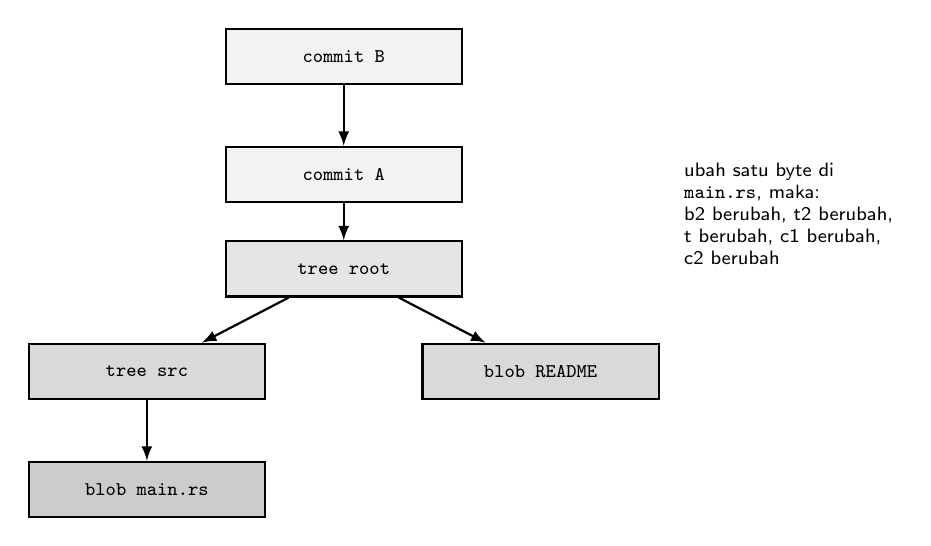
\begin{tikzpicture}[
			node distance=0.6cm and 1.2cm,
			nodebox/.style={rectangle, draw=black, thick, minimum width=3cm, minimum height=0.7cm, align=center, font=\ttfamily\scriptsize},
			line/.style={draw, thick, -latex}
		]
		\node[nodebox, fill=black!5] (c2) at (0, 3.5) {commit B};
		\node[nodebox, fill=black!5] (c1) at (0, 2.0) {commit A};
		\node[nodebox, fill=black!10] (t) at (0, 0.8) {tree root};
		\node[nodebox, fill=black!15] (t2) at (-2.5, -0.5) {tree src};
		\node[nodebox, fill=black!15] (b1) at (2.5, -0.5) {blob README};
		\node[nodebox, fill=black!20] (b2) at (-2.5, -2.0) {blob main.rs};

		\draw[line] (c2) -- (c1);
		\draw[line] (c1) -- (t);
		\draw[line] (t) -- (t2);
		\draw[line] (t) -- (b1);
		\draw[line] (t2) -- (b2);

		\node[font=\scriptsize\sffamily, anchor=west, align=left] at (4.2, 1.5) {ubah satu byte di\\\texttt{main.rs}, maka:\\b2 berubah, t2 berubah,\\t berubah, c1 berubah,\\c2 berubah};
	\end{tikzpicture}
	\caption{Pohon Merkle pada object store. Perubahan pada satu blob merambat sampai ke commit teratas.}
	\label{fig:merkle}
\end{figure}

Cara membaca Gambar~\ref{fig:merkle}: gambar ini menampilkan enam kotak bernama objek dengan panah dari anak ke induk. Blob main.rs di bawah, tree src di atasnya, lalu tree root, commit A, dan commit B di paling atas. Kotak blob README ada di sejajar tree src, juga bercabang ke tree root. Di sebelah kanan ada keterangan bahwa perubahan satu byte di main.rs merambat naik lewat setiap level. Inti pesan gambar ini adalah hash di level atas bergantung transitif pada hash di level bawah.

\subsection{Ringkasan Tipe Objek}

\begin{table}[H]
	\centering
	\caption{Ringkasan empat tipe objek dan hash.}
	\label{tab:types}
	\footnotesize
	\begin{tabularx}{\textwidth}{l X X}
		\toprule
		Tipe            & Isi utama               & Peran                                   \\
		\midrule
		\texttt{Blob}   & byte mentah satu file   & menyimpan isi tanpa nama                \\
		\texttt{Tree}   & daftar nama, mode, hash & memetakan nama ke isi                   \\
		\texttt{Commit} & tree, parent, metadata  & merekam snapshot dan sejarah            \\
		\texttt{Tag}    & target, tagger, pesan   & label permanen yang bisa ditandatangani \\
		\texttt{Hash}   & 64 byte hasil SHA-512   & alamat konten seluruh objek             \\
		\bottomrule
	\end{tabularx}
\end{table}

\section{Content Addressing dengan SHA-512}

\subsection{Mengapa Content Addressing, Bukan Address-Based}

Sistem berkas konvensional memberi alamat pada file berdasarkan nomor inode, path, atau offset. Alamat itu stabil selama file tidak dipindahkan, tetapi tidak memberi informasi apa pun tentang isi. Sistem kontrol versi membutuhkan tiga hal yang tidak bisa diberikan oleh alamat konvensional.

Pertama, deduplikasi. Jika dua commit menyimpan file identik, sistem tidak perlu menyimpannya dua kali. Dengan alamat berbasis isi, keduanya memiliki alamat yang sama, dan penyimpanan kedua tidak melakukan apa-apa.

Kedua, verifikasi integritas. Jika file di disk rusak, sistem bisa menghitung ulang hash dan membandingkannya dengan alamat. Ketidakcocokan menandakan korupsi.

Ketiga, immutability. Objek yang alamatnya ditentukan oleh isi tidak bisa diubah tanpa mengubah alamatnya. Sistem bisa mengasumsikan bahwa objek dengan alamat tertentu selalu memiliki isi yang sama, di mana pun dan kapan pun.

\subsection{Siklus Hidup Satu Objek}

Proses penyimpanan satu objek pada content-addressable storage mengikuti lima langkah tetap. Gambar~\ref{fig:cycle} menunjukkan siklusnya.

\begin{figure}[H]
	\centering
	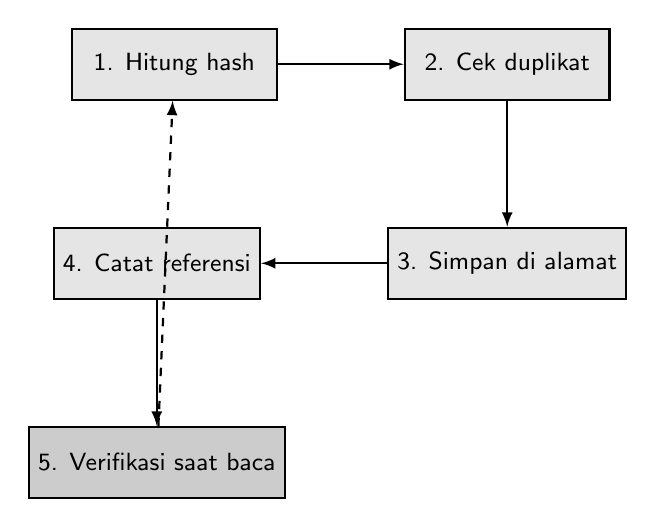
\begin{tikzpicture}[
			node distance=1.6cm,
			box/.style={rectangle, draw=black, thick, fill=black!10, minimum width=2.6cm, minimum height=0.9cm, align=center, font=\sffamily\small},
			line/.style={draw, thick, -latex}
		]
		\node[box] (hash) {1. Hitung hash};
		\node[box, right=of hash] (check) {2. Cek duplikat};
		\node[box, below=of check] (store) {3. Simpan di alamat};
		\node[box, left=of store] (index) {4. Catat referensi};
		\node[box, below=of index, fill=black!20] (verify) {5. Verifikasi saat baca};

		\draw[line] (hash) -- (check);
		\draw[line] (check) -- (store);
		\draw[line] (store) -- (index);
		\draw[line] (index) -- (verify);
		\draw[line, dashed] (verify) -- (hash);
	\end{tikzpicture}
	\caption{Siklus lima tahap penyimpanan objek pada content-addressable storage.}
	\label{fig:cycle}
\end{figure}

Cara membaca Gambar~\ref{fig:cycle}: gambar ini menampilkan lima kotak yang tersusun dalam pola empat di atas dan satu di bawah. Kotak pertama di kiri atas berlabel Hitung hash, kotak kedua di kanan atas berlabel Cek duplikat, kotak ketiga di kanan bawah berlabel Simpan di alamat, kotak keempat di kiri bawah berlabel Catat referensi, dan kotak kelima di bawah lagi berlabel Verifikasi saat baca. Panah mengalir dari kiri atas ke kanan atas, lalu turun, lalu ke kiri, lalu turun lagi. Ada panah putus-putus dari kotak kelima kembali ke kotak pertama. Inti pesan gambar ini adalah siklus penyimpanan berulang setiap kali objek dibaca kembali.

\subsection{Implementasi dengan SHA-512}

libvctrl memakai SHA-512, bukan SHA-256, karena SHA-512 pada perangkat 64-bit justru lebih cepat daripada SHA-256. Ukuran outputnya 64 byte, yang pas dengan \texttt{HASH\_LENGTH}. Tipe \texttt{Hash} di \texttt{libvctrl\_handler} adalah \texttt{[u8; 64]}.

\begin{lstlisting}[style=code]
use libvctrl::Hash;

let raw = [0xAB_u8; 64];
let hash = Hash::from_bytes(&raw)?;
println!("{}", hash);
\end{lstlisting}

\begin{lstlisting}[style=out]
ababababababababababababababababababababab
abababababababababababababababababababababab
\end{lstlisting}

Representasi hex untuk hash 64 byte selalu 128 karakter. Representasi ini dipakai pada output terminal dan pada nama file objek di disk.

\subsection{Pipeline Encode, Hash, Store, Decode}

Satu putaran penuh pada object store mengikuti pola tetap. Gambar~\ref{fig:roundtrip} menunjukkan pipeline-nya.

\begin{figure}[H]
	\centering
	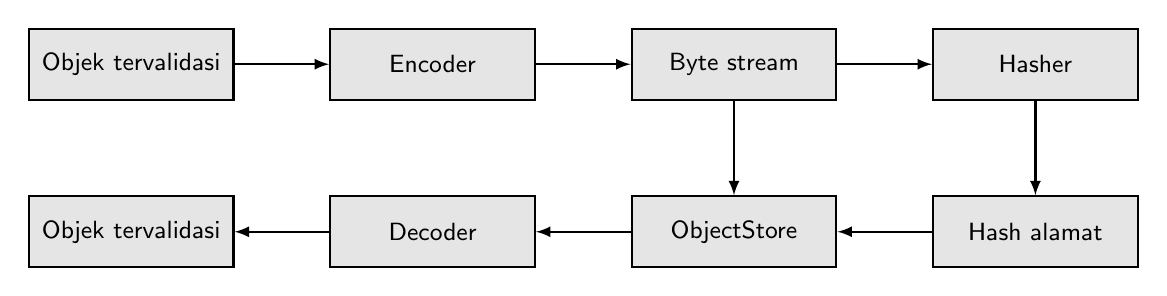
\begin{tikzpicture}[
			node distance=1.2cm,
			box/.style={rectangle, draw=black, thick, fill=black!10, minimum width=2.6cm, minimum height=0.9cm, align=center, font=\sffamily\small},
			line/.style={draw, thick, -latex}
		]
		\node[box] (obj) {Objek tervalidasi};
		\node[box, right=of obj] (enc) {Encoder};
		\node[box, right=of enc] (byt) {Byte stream};
		\node[box, right=of byt] (hash) {Hasher};
		\node[box, below=of hash] (hashv) {Hash alamat};
		\node[box, below=of byt] (st) {ObjectStore};
		\node[box, below=of enc] (dec) {Decoder};
		\node[box, below=of obj] (obj2) {Objek tervalidasi};

		\draw[line] (obj) -- (enc);
		\draw[line] (enc) -- (byt);
		\draw[line] (byt) -- (hash);
		\draw[line] (hash) -- (hashv);
		\draw[line] (hashv) -- (st);
		\draw[line] (byt) -- (st);
		\draw[line] (st) -- (dec);
		\draw[line] (dec) -- (obj2);
	\end{tikzpicture}
	\caption{Pipeline encode, hash, store, dan decode. Encoder dan Decoder adalah dua sisi dari kodek biner yang sama.}
	\label{fig:roundtrip}
\end{figure}

Cara membaca Gambar~\ref{fig:roundtrip}: gambar ini menampilkan empat kotak di baris atas dan empat kotak di baris bawah. Baris atas dari kiri ke kanan berisi Objek tervalidasi, Encoder, Byte stream, dan Hasher. Baris bawah dari kanan ke kiri berisi Hash alamat, ObjectStore, Decoder, dan Objek tervalidasi. Panah mengalir dari kiri atas ke kanan atas, lalu turun ke hash alamat, lalu ke object store, lalu ke decoder, lalu ke objek tervalidasi di kiri bawah. Inti pesan gambar ini adalah satu siklus penuh mengubah objek menjadi byte, byte menjadi hash, byte disimpan, lalu byte dibaca dan diubah kembali menjadi objek.

\subsection{Mengapa Hash Kriptografis, Bukan CRC}

CRC32 dan MD5 sengaja tidak dipakai. Alasannya ada tiga.

Pertama, tabrakan. CRC32 punya 32 bit, MD5 punya 128 bit tetapi sudah dianggap rusak untuk keperluan kriptografis. Untuk repositori dengan miliaran objek, tabrakan MD5 menjadi masalah nyata. SHA-512 punya 512 bit, cukup untuk seluruh repositori dalam beberapa abad.

Kedua, ketahanan terhadap upaya membalik. Untuk keperluan alamat, kita ingin fungsi hash yang tidak bisa dibalik tanpa memegang input aslinya. SHA-512 memenuhi syarat ini; CRC32 tidak.

Ketiga, ketahanan terhadap perubahan kecil. Perubahan satu bit pada input harus mengubah sekitar separuh output. SHA-512 memenuhi efek avalanche ini dengan baik; CRC32 juga memenuhinya, tetapi tidak cukup besar untuk mencegah tabrakan.

\subsection{Mengapa Batas Resource Wajib Ada}

Decoder membaca dari stream yang mungkin berasal dari input berbahaya. Tanpa batas, satu byte header bisa menyatakan bahwa blob berukuran 100 GB, dan proses akan mencoba mengalokasikan 100 GB sebelum menyadari bahwa stream sebenarnya hanya berisi 10 byte. Ini adalah serangan denial-of-service klasik.

libvctrl menambahkan batas keras pada seluruh tipe objek. Tabel~\ref{tab:limits} merangkumnya.

\begin{table}[H]
	\centering
	\caption{Konstanta batas resource pada \texttt{libvctrl\_handler}.}
	\label{tab:limits}
	\footnotesize
	\begin{tabularx}{\textwidth}{l r X}
		\toprule
		Konstanta                     & Nilai    & Tujuan                        \\
		\midrule
		\texttt{HASH\_LENGTH}         & 64 byte  & ukuran hash SHA-512           \\
		\texttt{MAX\_NAME\_LENGTH}    & 255 byte & batas nama file dan referensi \\
		\texttt{MAX\_BLOB\_SIZE}      & 100 MiB  & DoS breaker pada blob         \\
		\texttt{MAX\_TREE\_ENTRIES}   & 100 ribu & batas jumlah entri per tree   \\
		\texttt{MAX\_MESSAGE\_LENGTH} & 1 MiB    & batas pesan commit dan tag    \\
		\texttt{MAX\_PARENT\_COUNT}   & 65535    & batas parent (u16)            \\
		\bottomrule
	\end{tabularx}
\end{table}

Setiap batas dipaksakan di konstruktor. Blob yang terlalu besar tidak bisa dibuat; tree yang terlalu panjang tidak bisa dirakit; commit dengan terlalu banyak parent ditolak dengan \texttt{ExceededMaxSize}. Pemaksaan di konstruktor berarti objek yang melewati batas tidak pernah ada di sistem.

\subsection{Immutability sebagai Konsekuensi}

Immutability bukan fitur yang ditambahkan; ia adalah konsekuensi langsung dari alamat berbasis hash. Jika objek dengan alamat H bisa diubah isinya, maka hash dari isi yang baru tidak akan sama dengan H, dan alamat itu tidak lagi merujuk objek tersebut. Dengan kata lain, "mengubah objek" berarti "membuat objek baru dengan alamat baru"; objek lama tetap ada dengan alamat lamanya. Gambar~\ref{fig:immut} menyandingkan sifat mutable dan immutable pada sistem penyimpanan.

\begin{figure}[H]
	\centering
	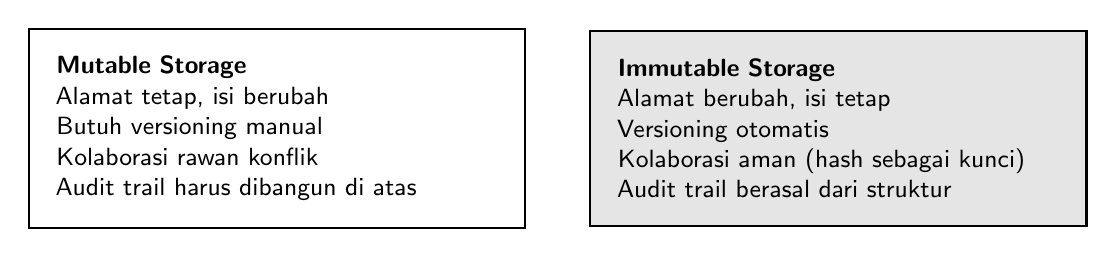
\begin{tikzpicture}[
			box/.style={rectangle, draw=black, thick, text width=5.6cm, align=left, font=\sffamily\small, inner sep=10pt}
		]
		\node[box, fill=white] (a) {
			\textbf{Mutable Storage} \\
			Alamat tetap, isi berubah \\
			Butuh versioning manual \\
			Kolaborasi rawan konflik \\
			Audit trail harus dibangun di atas
		};
		\node[box, fill=black!10, right=0.8cm of a] (b) {
			\textbf{Immutable Storage} \\
			Alamat berubah, isi tetap \\
			Versioning otomatis \\
			Kolaborasi aman (hash sebagai kunci) \\
			Audit trail berasal dari struktur
		};
	\end{tikzpicture}
	\caption{Perbandingan mutable dan immutable storage.}
	\label{fig:immut}
\end{figure}

Cara membaca Gambar~\ref{fig:immut}: gambar ini menampilkan dua kotak sejajar. Kotak kiri berlabel Mutable Storage dengan empat poin: alamat tetap isi berubah, butuh versioning manual, kolaborasi rawan konflik, audit trail harus dibangun di atas. Kotak kanan berlabel Immutable Storage dengan empat poin berlawanan: alamat berubah isi tetap, versioning otomatis, kolaborasi aman dengan hash sebagai kunci, audit trail berasal dari struktur. Kotak kiri berlatar putih dan kotak kanan berlatar abu-abu muda. Inti pesan gambar ini adalah dua sifat penyimpanan yang berlawanan dan konsekuensinya pada versioning, kolaborasi, dan audit trail.

\section{Kodek Biner dan Backend Penyimpanan}

\subsection{Mengapa Kodek Biner, Bukan JSON}

Menulis objek VCS sebagai JSON terlihat menggoda karena mudah dibaca manusia dan mudah diparse. Tetapi ada tiga alasan mengapa libvctrl memakai kodek biner.

Pertama, determinisme. JSON tidak mendefinisikan urutan key, whitespace, dan representasi float. Dua serializer JSON dapat menghasilkan byte yang berbeda untuk objek yang sama, dan hash dari dua hasil itu akan berbeda. Kodek biner libvctrl menetapkan setiap field dengan urutan tetap, integer little-endian, dan string dengan prefix panjang. Byte hasil encode deterministik.

Kedua, ukuran. JSON membawa banyak karakter tambahan: kurung kurawal, tanda kutip, koma, dan nama field yang diulang setiap objek. Kodek biner tidak. Untuk repositori dengan jutaan objek, selisih ini menjadi ratusan megabyte.

Ketiga, tipe. JSON tidak membedakan integer dengan string, dan tidak membedakan byte biner dengan string UTF-8. Kodek biner libvctrl menetapkan tipe setiap field, sehingga decoder dapat menolak input yang salah tipe sebelum sampai ke konstruktor.

\subsection{Header Versioning}

Setiap objek yang dikodekan dimulai dengan satu byte version. Byte ini wajib bernilai 3 pada implementasi saat ini. Decoder menolak input yang byte pertamanya tidak bernilai 3, sehingga format bisa berubah di masa depan tanpa harus mempertahankan kompatibilitas mundur pada decoder yang sama.

\begin{lstlisting}[style=code]
use libvctrl::{Blob, Encoder, BinaryEncoder};

let blob = Blob::new(b"abc".to_vec())?;
let mut buf = Vec::new();
BinaryEncoder.encode_blob(&blob, &mut buf)?;
println!("bytes = {:?}", buf);
\end{lstlisting}

\begin{lstlisting}[style=out]
bytes = [3, 3, 0, 0, 0, 0, 0, 0, 0, 97, 98, 99]
\end{lstlisting}

Byte pertama adalah version (3). Delapan byte berikutnya adalah panjang data dalam little-endian (3). Tiga byte terakhir adalah isi data itu sendiri (a, b, c). Total dua belas byte. Format ini berbeda dari Git yang memakai format teks header bertipe ("blob 3\x00abc"), dan perbedaan ini disengaja agar proses decode tidak perlu memindai untuk menemukan batas header.

\subsection{Mengimplementasikan ObjectStore Sendiri}

Salah satu klaim utama arsitektur libvctrl adalah backend bisa diganti. Untuk membuktikan klaim itu, cukup mengimplementasikan empat method dari trait \texttt{ObjectStore}.

\begin{lstlisting}[style=code]
use std::io::{self, Read};
use libvctrl::{Hash, ObjectStore, VctrlError};

struct NullStore;

impl ObjectStore for NullStore {
    fn put(&mut self, _h: &Hash, _d: &[u8]) -> Result<(), VctrlError> {
        Ok(())
    }
    fn get(&self, _h: &Hash)
        -> Result<Box<dyn Read + Send + '_>, VctrlError>
    {
        Ok(Box::new(io::empty()))
    }
    fn delete(&mut self, _h: &Hash) -> Result<(), VctrlError> {
        Ok(())
    }
    fn exists(&self, _h: &Hash) -> Result<bool, VctrlError> {
        Ok(false)
    }
}
\end{lstlisting}

Implementasi ini tidak menyimpan apa pun, tetapi ia memenuhi kontrak dan dapat diserahkan ke \texttt{Repository::new} tanpa perubahan kode lain. Pengujian bisa memakai \texttt{NullStore} untuk memverifikasi alur tanpa menyentuh filesystem.

\subsection{Backend Monumentum}

\texttt{libvctrl\_monumentum} adalah backend alternatif yang menyimpan objek di mesin \texttt{monumentum}. Ia mengimplementasikan dua trait (\texttt{ObjectStore} dan \texttt{RefStore}) dengan memetakan hash dan data ke tabel-tabel \texttt{monumentum}. Pemakai \texttt{Repository} tidak perlu tahu perbedaan antara \texttt{MemoryStore}, \texttt{MonumentumStore}, dan backend kustom; semuanya diserahkan sebagai \texttt{Box<dyn ObjectStore>}.

Pola ini adalah alasan utama arsitektur berlapis: seseorang yang ingin menyimpan objek di PostgreSQL, SQLite, atau S3 tidak perlu menulis ulang \texttt{Repository}. Ia cukup mengimplementasikan trait.

\subsection{Ringkasan Format Kodek}

\begin{table}[H]
	\centering
	\caption{Ringkasan format kodek biner versi 3.}
	\label{tab:codec}
	\footnotesize
	\begin{tabularx}{\textwidth}{l X}
		\toprule
		Field          & Format                                  \\
		\midrule
		Version        & 1 byte, wajib bernilai 3                \\
		Hash           & 64 byte (SHA-512)                       \\
		Integer        & little-endian                           \\
		Panjang        & u8, u16, u32, atau u64 sesuai kebutuhan \\
		String         & prefix panjang (u8 atau u32) + UTF-8    \\
		Tree entry     & panjang nama + nama + kind + hash       \\
		Commit parent  & u16 jumlah + hash per parent            \\
		Optional field & 1 byte penanda + isi jika ada           \\
		\bottomrule
	\end{tabularx}
\end{table}

\section{Perbandingan dan Sintesis}

Setelah memahami tujuh lapisan, model objek, content addressing, dan kodek, seluruh keputusan arsitektur dapat diringkas dalam satu tabel. Tabel~\ref{tab:synth} menyandingkan tujuh aspek.

\begin{table}[H]
	\centering
	\caption{Sintesis keputusan arsitektur libvctrl.}
	\label{tab:synth}
	\footnotesize
	\begin{tabularx}{\textwidth}{l X X}
		\toprule
		Aspek           & Keputusan                         & Alasan                            \\
		\midrule
		Lapisan         & tujuh crate terpisah              & pengujian dan penggantian backend \\
		Arah dependensi & satu arah, tanpa siklus           & isolasi perubahan                 \\
		Kontrak         & trait + tipe immutable            & jaminan konstruktor               \\
		Validasi        & konstruktor fallible              & invalid state tidak ada           \\
		Alamat          & SHA-512 atas byte encode          & deduplikasi + integritas          \\
		Format          & biner little-endian deterministik & hash stabil, ukuran kecil         \\
		Batas resource  & konstanta MAX di konstruktor      & DoS dicegah sebelum alokasi       \\
		Backend         & trait ObjectStore + RefStore      & penggantian tanpa ubah pengguna   \\
		\bottomrule
	\end{tabularx}
\end{table}

Dua paragraf penutup dari perbandingan ini. Pertama, setiap keputusan adalah respons terhadap masalah konkret, bukan preferensi estetika. Batas resource ada karena serangan DoS pernah terjadi. Format biner ada karena hash stabil butuh determinisme. Kontrak trait ada karena backend SQLite perlu ditambahkan tanpa menyentuh kode perintah.

Kedua, keputusan-keputusan ini saling memperkuat. Format biner deterministik hanya berguna jika tipe data immutable; tipe immutable hanya berguna jika kontrak dipaksakan di konstruktor; kontrak dipaksakan hanya berguna jika tidak ada jalan pintas lewat trait yang sama. Rantai ini adalah alasan arsitektur berlapis bukan sekadar kosmetik.

\section{Studi Kasus: Menyimpan Commit Pertama}

Bagian ini mengikuti delapan langkah menyimpan satu commit di libvctrl, dimulai dari byte mentah sampai referensi yang bisa dibaca kembali.

\subsection{Langkah 1: Menyiapkan Isi File}

Isi file disiapkan sebagai byte stream. Nama file disimpan terpisah; blob hanya berisi isi.

\begin{lstlisting}[style=code]
let content: Vec<u8> = b"hello, vcs\n".to_vec();
println!("content len = {}", content.len());
\end{lstlisting}

\begin{lstlisting}[style=out]
content len = 11
\end{lstlisting}

\subsection{Langkah 2: Membangun Blob Tervalidasi}

Blob dibangun lewat konstruktor fallible. Jika isi melebihi 100 MiB, konstruksi gagal sebelum alokasi besar terjadi.

\begin{lstlisting}[style=code]
use libvctrl::Blob;

let blob = Blob::new(content)?;
println!("blob size = {}", blob.size());
\end{lstlisting}

\begin{lstlisting}[style=out]
blob size = 11
\end{lstlisting}

\subsection{Langkah 3: Mengencode Blob ke Byte Stream}

Blob diubah menjadi byte stream deterministik dengan header version. Byte stream inilah yang akan di-hash dan disimpan.

\begin{lstlisting}[style=code]
use libvctrl::{BinaryEncoder, Encoder};

let mut blob_bytes = Vec::new();
BinaryEncoder.encode_blob(&blob, &mut blob_bytes)?;
println!("encoded len = {}", blob_bytes.len());
\end{lstlisting}

\begin{lstlisting}[style=out]
encoded len = 20
\end{lstlisting}

\subsection{Langkah 4: Menghitung Hash dan Menyimpan Blob}

Hash dihitung atas byte stream, bukan atas isi file. Byte stream inilah yang disimpan di object store dengan kunci hash.

\begin{lstlisting}[style=code]
use libvctrl::{Hasher, MemoryStore, ObjectStore, Sha512Hasher};

let blob_hash = Sha512Hasher.hash(blob_bytes.as_slice())?;
let mut store = MemoryStore::new();
store.put(&blob_hash, &blob_bytes)?;
println!("stored blob {}", blob_hash);
\end{lstlisting}

\begin{lstlisting}[style=out]
stored blob 4a8b1c...be7f
\end{lstlisting}

\subsection{Langkah 5: Membangun Tree dengan Satu Entri}

Tree menyimpan nama file, mode, dan hash blob. Nama file tinggal di tree, bukan di blob.

\begin{lstlisting}[style=code]
use libvctrl::{EntryKind, Tree, TreeEntry};

let entry = TreeEntry::new(
    "hello.txt".to_string(),
    EntryKind::Blob,
    blob_hash,
)?;
let tree = Tree::new(vec![entry])?;
println!("tree entries = {}", tree.len());
\end{lstlisting}

\begin{lstlisting}[style=out]
tree entries = 1
\end{lstlisting}

\subsection{Langkah 6: Mengencode dan Menghash Tree}

Tree diencode, di-hash, dan disimpan dengan pola yang sama seperti blob.

\begin{lstlisting}[style=code]
let mut tree_bytes = Vec::new();
BinaryEncoder.encode_tree(&tree, &mut tree_bytes)?;
let tree_hash = Sha512Hasher.hash(tree_bytes.as_slice())?;
store.put(&tree_hash, &tree_bytes)?;
println!("tree {}", tree_hash);
\end{lstlisting}

\begin{lstlisting}[style=out]
tree 8f3a5d...c0e2
\end{lstlisting}

\subsection{Langkah 7: Membangun Commit}

Commit menyimpan hash tree, daftar parent (kosong untuk commit pertama), author, committer, dan pesan. Metadata timestamp dan timezone disimpan dalam \texttt{CommitMeta}.

\begin{lstlisting}[style=code]
use libvctrl::{Commit, CommitMeta, UserID};

let user = UserID::new(
    "Alice".to_string(),
    "alice@example.com".to_string(),
)?;
let meta = CommitMeta::new(1_700_000_000, 0, None)?;
let commit = Commit::with_meta(
    tree_hash,
    vec![],
    user.clone(),
    user,
    "first commit\n".to_string(),
    meta,
)?;
\end{lstlisting}

\subsection{Langkah 8: Mengencode Commit dan Memperbarui Referensi}

Commit diencode, di-hash, disimpan, lalu referensi \texttt{refs/heads/main} diperbarui agar menunjuk ke hash commit. Setelah langkah ini, seluruh isi repositori dapat dibaca kembali dari referensi.

\begin{lstlisting}[style=code]
use libvctrl::MemoryRefStore;

let mut commit_bytes = Vec::new();
BinaryEncoder.encode_commit(&commit, &mut commit_bytes)?;
let commit_hash = Sha512Hasher.hash(commit_bytes.as_slice())?;
store.put(&commit_hash, &commit_bytes)?;

let mut refs = MemoryRefStore::new();
refs.set_ref("refs/heads/main", &commit_hash)?;
println!("HEAD -> {}", refs.get_ref("refs/heads/main")?);
\end{lstlisting}

\begin{lstlisting}[style=out]
HEAD -> 7d2e9a...41bc
\end{lstlisting}

\subsection{Timeline Studi Kasus}

Gambar~\ref{fig:timeline} merangkum delapan langkah dalam satu garis waktu.

\begin{figure}[H]
	\centering
	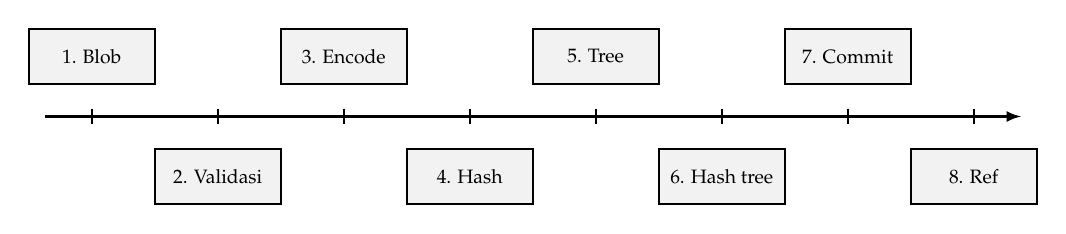
\begin{tikzpicture}[
			ev/.style={rectangle, draw=black, thick, fill=black!5, minimum width=1.6cm, minimum height=0.7cm, align=center, font=\scriptsize},
			line/.style={draw, thick}
		]
		\draw[line, -latex] (-6.2, 0) -- (6.2, 0);

		\draw[thick] (-5.6, 0.1) -- (-5.6, -0.1);
		\node[ev, above=0.2cm] at (-5.6, 0.2) {1. Blob};

		\draw[thick] (-4.0, 0.1) -- (-4.0, -0.1);
		\node[ev, below=0.2cm] at (-4.0, -0.2) {2. Validasi};

		\draw[thick] (-2.4, 0.1) -- (-2.4, -0.1);
		\node[ev, above=0.2cm] at (-2.4, 0.2) {3. Encode};

		\draw[thick] (-0.8, 0.1) -- (-0.8, -0.1);
		\node[ev, below=0.2cm] at (-0.8, -0.2) {4. Hash};

		\draw[thick] (0.8, 0.1) -- (0.8, -0.1);
		\node[ev, above=0.2cm] at (0.8, 0.2) {5. Tree};

		\draw[thick] (2.4, 0.1) -- (2.4, -0.1);
		\node[ev, below=0.2cm] at (2.4, -0.2) {6. Hash tree};

		\draw[thick] (4.0, 0.1) -- (4.0, -0.1);
		\node[ev, above=0.2cm] at (4.0, 0.2) {7. Commit};

		\draw[thick] (5.6, 0.1) -- (5.6, -0.1);
		\node[ev, below=0.2cm] at (5.6, -0.2) {8. Ref};
	\end{tikzpicture}
	\caption{Timeline delapan langkah menyimpan commit pertama.}
	\label{fig:timeline}
\end{figure}

Cara membaca Gambar~\ref{fig:timeline}: gambar ini menampilkan garis horizontal dengan panah ke kanan. Di sepanjang garis ada delapan tanda dan kotak kecil dengan label bernomor. Kotak label bergantian posisi: satu di atas garis, satu di bawah garis. Nomor dan label: satu Blob, dua Validasi, tiga Encode, empat Hash, lima Tree, enam Hash tree, tujuh Commit, delapan Ref. Inti pesan gambar ini adalah alur linear dari byte mentah sampai referensi.

\begin{table}[H]
	\centering
	\caption{Ringkasan delapan langkah studi kasus.}
	\label{tab:case}
	\footnotesize
	\begin{tabularx}{\textwidth}{l X X}
		\toprule
		Langkah & Operasi                & Hasil                                 \\
		\midrule
		1       & siapkan isi file       & 11 byte mentah                        \\
		2       & bangun \texttt{Blob}   & blob tervalidasi                      \\
		3       & encode \texttt{Blob}   & 20 byte dengan header version         \\
		4       & hash dan simpan        & blob tersimpan dengan kunci hash      \\
		5       & bangun \texttt{Tree}   & tree dengan satu entri                \\
		6       & encode dan hash tree   & tree tersimpan dengan kunci hash      \\
		7       & bangun \texttt{Commit} & commit dengan satu tree, tanpa parent \\
		8       & encode, hash, set ref  & referensi menunjuk hash commit        \\
		\bottomrule
	\end{tabularx}
\end{table}

\section{Kesalahan Umum dan Cara Menghindarinya}

\begin{table}[H]
	\centering
	\caption{Kesalahan umum saat memakai atau membangun di atas libvctrl.}
	\label{tab:mistakes}
	\footnotesize
	\begin{tabularx}{\textwidth}{l X X}
		\toprule
		Kesalahan                                    & Akibat                                   & Perbaikan                                       \\
		\midrule
		hash data file mentah, bukan byte encode     & hash tidak cocok dengan hash objek       & hash selalu atas byte encode                    \\
		menyimpan blob sebelum menghitung hash       & objek tidak bisa ditemukan kembali       & hitung hash dulu, lalu simpan                   \\
		membuat tree tanpa mengurutkan entri         & hash berbeda untuk isi sama              & pakai \texttt{Tree::new} yang sudah mengurutkan \\
		memakai \texttt{HashMap<String>} untuk hash  & alokasi berlebih dan lambat              & pakai \texttt{Hash} yang \texttt{Copy}          \\
		membaca stream tanpa batas                   & DoS dari input berbahaya                 & andalkan \texttt{read\_bounded} di decoder      \\
		menyimpan objek kosong tanpa cek batas       & alokasi kecil tak terbatas               & \texttt{Blob::new} sudah menolak melebihi batas \\
		melewati \texttt{VctrlError}                 & informasi hilang di lapisan atas         & teruskan error apa adanya                       \\
		memakai \texttt{unwrap} di luar pengujian    & panic pada input tidak valid             & pakai \texttt{?} untuk propagasi                \\
		menulis backend tanpa \texttt{Send}          & backend tidak bisa dipakai lintas thread & tambahkan bound \texttt{Send + Sync}            \\
		mengganti \texttt{Hash} jadi \texttt{String} & hash 128 byte per objek, bukan 64        & pakai tipe \texttt{Hash}                        \\
		\bottomrule
	\end{tabularx}
\end{table}

Dua kesalahan yang paling sering muncul adalah menghitung hash atas isi file mentah dan memakai \texttt{String} sebagai kunci hash. Yang pertama membuat deduplikasi gagal; file yang sama tetapi dengan metadata berbeda menghasilkan hash berbeda, sehingga dua salinan disimpan. Yang kedua membuat setiap lookup dan perbandingan memakan dua kali ruang; untuk repositori dengan dua puluh juta objek, selisih ini menjadi lebih dari satu gigabyte.

\section{Lembar Rujukan Cepat}

\begin{table}[H]
	\centering
	\caption{Lembar rujukan cepat untuk bekerja dengan libvctrl.}
	\label{tab:cheat}
	\footnotesize
	\begin{tabularx}{\textwidth}{l X}
		\toprule
		Kebutuhan                    & Perintah atau tipe                    \\
		\midrule
		tambah dependensi fasad      & \texttt{libvctrl = "2.2"}             \\
		tambah dependensi kontrak    & \texttt{libvctrl\_handler = "5.2"}    \\
		tambah dependensi kripto     & \texttt{libvctrl\_sha512 = "3.2"}     \\
		bangun blob                  & \texttt{Blob::new(bytes)?}            \\
		bangun tree                  & \texttt{Tree::new(entries)?}          \\
		bangun commit                & \texttt{Commit::with\_meta(...)?}     \\
		bangun tag                   & \texttt{Tag::with\_meta(...)?}        \\
		encode blob                  & \texttt{BinaryEncoder.encode\_blob}   \\
		encode tree                  & \texttt{BinaryEncoder.encode\_tree}   \\
		encode commit                & \texttt{BinaryEncoder.encode\_commit} \\
		decode blob                  & \texttt{BinaryDecoder.decode\_blob}   \\
		hash byte stream             & \texttt{Sha512Hasher.hash(reader)}    \\
		simpan objek in-memory       & \texttt{MemoryStore.put}              \\
		baca objek in-memory         & \texttt{MemoryStore.get}              \\
		simpan referensi             & \texttt{MemoryRefStore.set\_ref}      \\
		implementasi backend sendiri & \texttt{impl ObjectStore for MyStore} \\
		implementasi ref sendiri     & \texttt{impl RefStore for MyStore}    \\
		cek hash hex                 & \texttt{format!("{}", hash)}          \\
		baca hash dari hex           & \texttt{hash.parse::<Hash>()}         \\
		kompilasi seluruh workspace  & \texttt{cargo test --workspace}       \\
		lint seluruh workspace       & \texttt{cargo clippy -- -D warnings}  \\
		\bottomrule
	\end{tabularx}
\end{table}

\section{Kesimpulan}

Arsitektur berlapis adalah pola yang memisahkan aturan dari implementasi, dan libvctrl mewujudkannya dalam tujuh crate yang masing-masing hanya bergantung ke lapisan di bawahnya. Lapisan kontrak (\texttt{libvctrl\_handler}) mendefinisikan apa itu blob, tree, commit, tag, dan hash tanpa menyebut cara menyimpannya. Lapisan implementasi referensi (\texttt{libvctrl\_core}) mengisi kontrak dengan kodek biner dan penyimpanan in-memory. Lapisan kripto (\texttt{libvctrl\_sha512}) memberi alamat berbasis isi yang membuat deduplikasi dan verifikasi integritas menjadi bawaan. Lapisan fasad menyatukan ketiganya; lapisan plumbing dan porcelain memberi perintah; lapisan backend alternatif membuktikan bahwa penggantian backend tidak perlu menyentuh kode pengguna.

Tiga prinsip penutup:

\begin{enumerate}
	\item Kontrak adalah fondasi, bukan dokumentasi. Setiap trait di \texttt{libvctrl\_handler} harus bisa diimplementasikan oleh crate mana pun tanpa menyentuh crate lain. Jika sebuah trait memaksa pemakai untuk menyentuh \texttt{libvctrl\_core}, berarti pemisahan kontrak dari implementasi belum tercapai.
	\item Alamat adalah isi. Jika dua objek harus dianggap sama, mereka harus memiliki alamat yang sama. Jika mereka harus berbeda, alamatnya harus berbeda. Aturan ini menghilangkan hampir semua kerumitan yang biasanya muncul pada sistem deduplikasi manual.
	\item Uji di batas, bukan di tengah. Pengujian yang paling berharga adalah pengujian pada konstruktor dan pada decoder, karena di situlah input tidak tepercaya masuk. Pengujian di tengah (misalnya pada perintah porcelain) hanya menguji orkestrasi, bukan kebenaran.
\end{enumerate}

Dengan kerangka ini, pembaca siap membaca kode sumber libvctrl, membangun VCS kecil sendiri di atas model yang sama, atau menambahkan backend baru tanpa menyentuh lapisan yang sudah stabil.

\newpage
\section*{Referensi}
\addcontentsline{toc}{section}{Referensi}

\begin{thebibliography}{99}

	\bibitem{klabnik}
	Klabnik, S., \& Nichols, C. (2019).
	\textit{The Rust Programming Language}.
	No Starch Press.
	\texttt{https://doc.rust-lang.org/book/}

	\bibitem{chacon}
	Chacon, S., \& Straub, B. (2014).
	\textit{Pro Git} (2nd ed.).
	Apress.
	\texttt{https://git-scm.com/book/}

	\bibitem{merkle}
	Merkle, R. C. (1988).
	A Digital Signature Based on a Conventional Encryption Function.
	In \textit{Advances in Cryptology --- CRYPTO '87}
	(pp. 369--378). Springer.

	\bibitem{nist}
	NIST. (2015).
	\textit{Secure Hash Standard (SHS)} (FIPS PUB 180-4).
	National Institute of Standards and Technology.
	\texttt{https://doi.org/10.6028/NIST.FIPS.180-4}

	\bibitem{api-guidelines}
	The Rust Project Developers. (2026).
	\textit{Rust API Guidelines}.
	\texttt{https://rust-lang.github.io/api-guidelines/}

	\bibitem{martin}
	Martin, R. C. (2017).
	\textit{Clean Architecture: A Craftsman's Guide to Software Structure and Design}.
	Prentice Hall.

	\bibitem{sommerville}
	Sommerville, I. (2016).
	\textit{Software Engineering} (10th ed.).
	Pearson.

	\bibitem{libvctrl}
	Khafidi, M. R. (2026).
	\textit{libvctrl: A Precision Toolkit for Building Custom Version Control Systems}.
	GitHub.
	\texttt{https://github.com/mroczect/libvctrl}

\end{thebibliography}

\end{document}
